\documentclass[10pt,letterpaper,final]{article}
\usepackage[left=4cm,rigth=4cm,top=4cm,bottom=4cm]{geometry}
\usepackage[utf8]{inputenc}
\usepackage{amsmath}
\usepackage{amsfonts}
\usepackage{amssymb}
\usepackage{graphicx}
\usepackage{kpfonts}
\usepackage{tabularx}
\usepackage{hyperref}
\usepackage{natbib}
\begin{document}
    \section*{}
    Rubén Martínez González
    \section*{Problematic of thesis}
    \begin{figure}[!ht]
        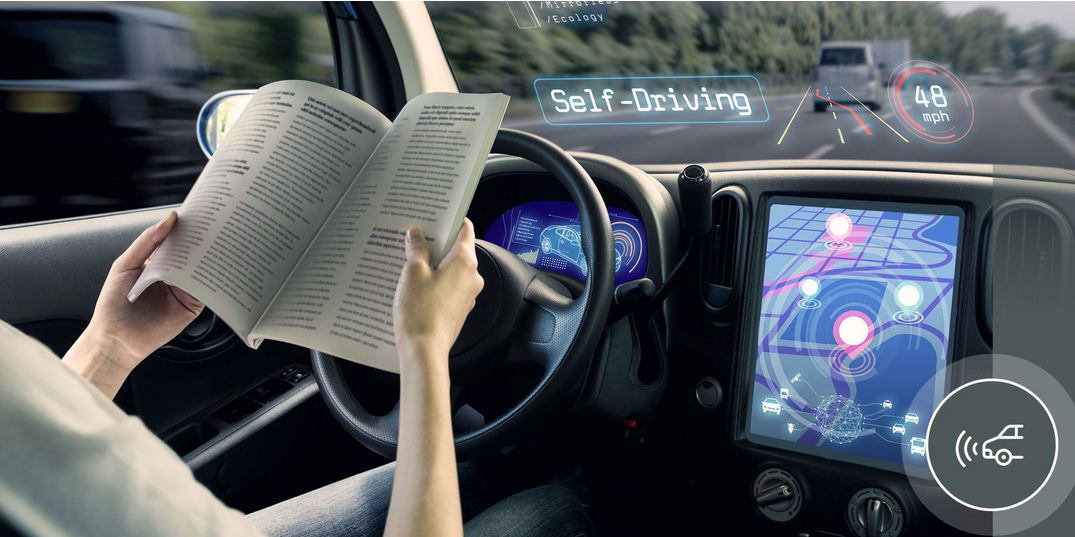
\includegraphics[width=\textwidth]{img/1}\label{fig:self-driving}
    \end{figure}
    \newline
    \noindent Se propone una investigación que aborde el ámbito de los vehículos autónomos:\\
    La necesidad de desarrollar sistemas ‘inteligentes' que permitan a estos vehículos aprender a conducir de manera autónoma y,
    al mismo tiempo, detectar posibles colisiones y reaccionar de manera similar a como lo haría un conductor humano.\\
    Esta problemática adquiere una relevancia crítica en la medida en que la adopción de vehículos autónomos en nuestras
    vías se acelera. Si bien los avances en la conducción autónoma han sido significativos, la detección y respuesta a
    situaciones de peligro, como colisiones inminentes, siguen siendo un desafío complejo.\\
    La seguridad en la carretera y la confianza del público en esta tecnología dependen en gran medida de la capacidad
    de los vehículos autónomos para enfrentar situaciones de tráfico de manera eficiente y segura.\\
    Esta investigación busca abordar esta problemática crítica, avanzando hacia un futuro en el que los vehículos autónomos
    sean capaces de igualar e incluso superar las habilidades de conducción humana en términos de detección y respuesta
    a situaciones de colisión.
    \clearpage

    \section*{Related Works}
    \newline
    \begin{longtable}
        \hline
        \noindent \textbf{Referencia:}~\cite{alam2022cost} \\
        \textbf{Título:} \\
        Autonomous Driving Architectures: Insights of Machine Learning and Deep Learning Algorithms \\
        \textbf{Autores:}
        Bachute, Mrinal R and Subhedar, Javed M \\
        \textbf{Año:}
        2021 \\
        \textbf{Revista:}
        Machine Learning with Applications \\
        \textbf{URL:}
        \url{https://www.sciencedirect.com/science/article/pii/S2666827021000827}
        \textbf{Resumen:}
        \begin{itemize}
            \item El artículo ofrece una visión general de cómo se aplican algoritmos de Aprendizaje Automático y Aprendizaje
            Profundo en sistemas de conducción autónoma y se enfoca en la evaluación de su desempeño en diversas tareas clave.
            \item Se centra en la investigación en el campo de la conducción autónoma y destaca que esta área está ganando
            impulso debido a las ventajas inherentes de los sistemas de conducción autónoma.
            \item Ventajas de la conducción autónoma, como la reducción de la intervención humana y la disociación del conductor del vehículo.
            \item La complejidad de los sistemas de conducción autónoma, que involucra la integración de múltiples subsistemas.
            \item Se analizan diversas tareas en la conducción autónoma, incluyendo la planificación de movimiento, la localización del vehículo,
            la detección de peatones, la detección de señales de tráfico, la detección de marcas viales, el estacionamiento automatizado,
            la ciberseguridad del vehículo y el diagnóstico de fallas del sistema.
            \item Uso de algoritmos de Aprendizaje Automático y Aprendizaje Profundo en arquitecturas de conducción autónoma para realizar estas tareas.
            \item Evaluación y comparación de algoritmos basada en métricas como mIoU, AP, tasa de detección perdida, tasa de omisión,
            falsos positivos por imagen y promedio de detección de fotogramas falsos.
        \end{itemize}

        \begin{figure}[!ht]
            \begin{subfigure}
                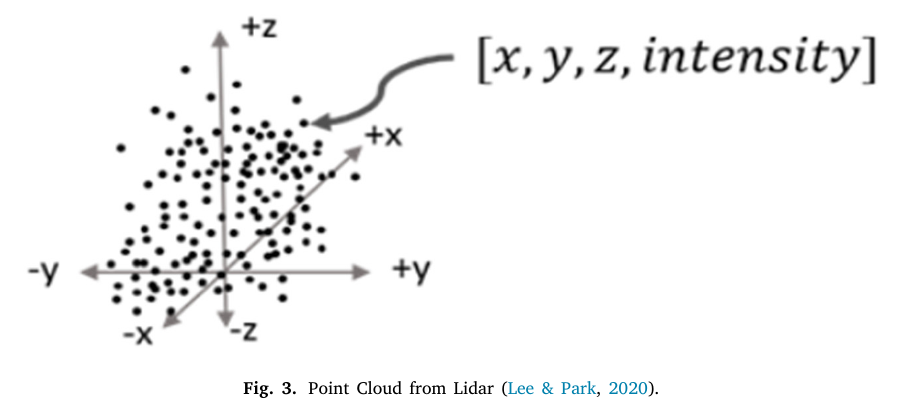
\includegraphics[width=0.5\textwidth]{img/1- Screenshot_20231106_142913}\label{fig:11}
            \end{subfigure}
            \begin{subfigure}
                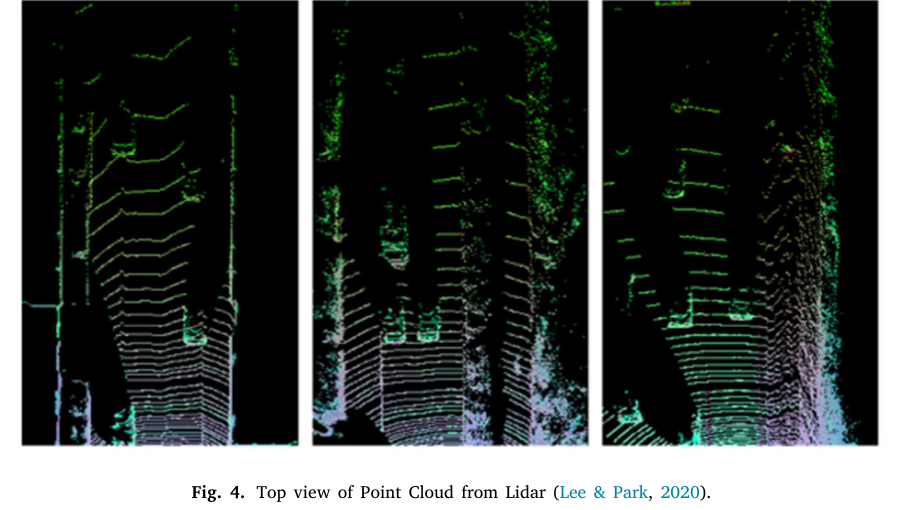
\includegraphics[width=0.5\textwidth]{img/12Screenshot_20231106_142954}\label{fig:12}
            \end{subfigure}
            \begin{subfigure}
                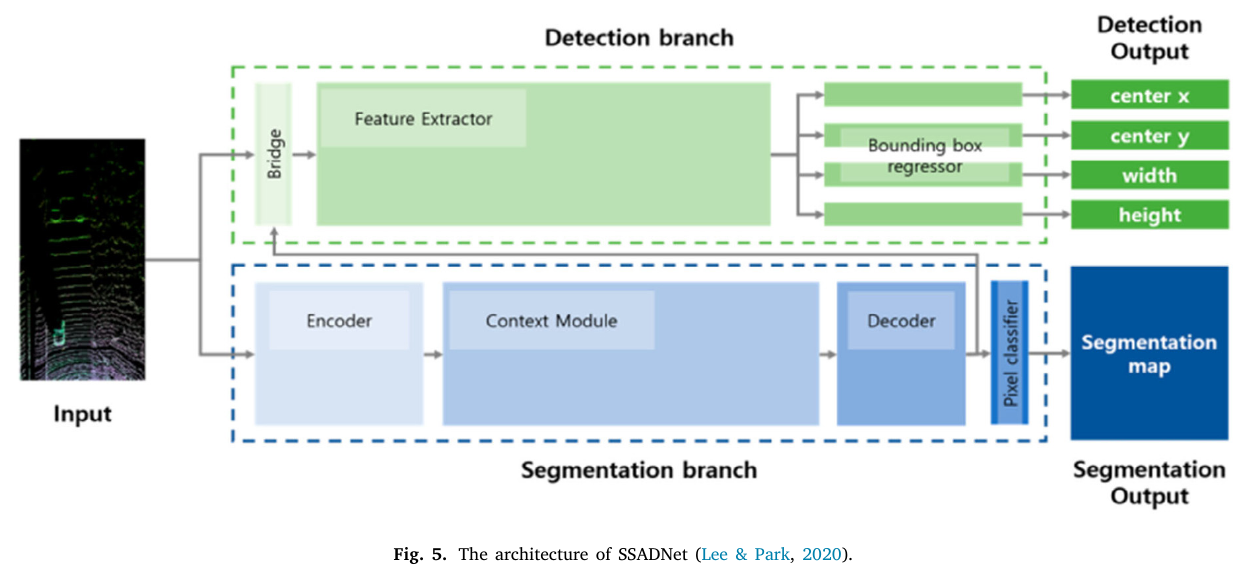
\includegraphics[width=0.6\textwidth]{img/13Screenshot_20231106_143018}\label{fig:13}
            \end{subfigure}
            \begin{subfigure}
                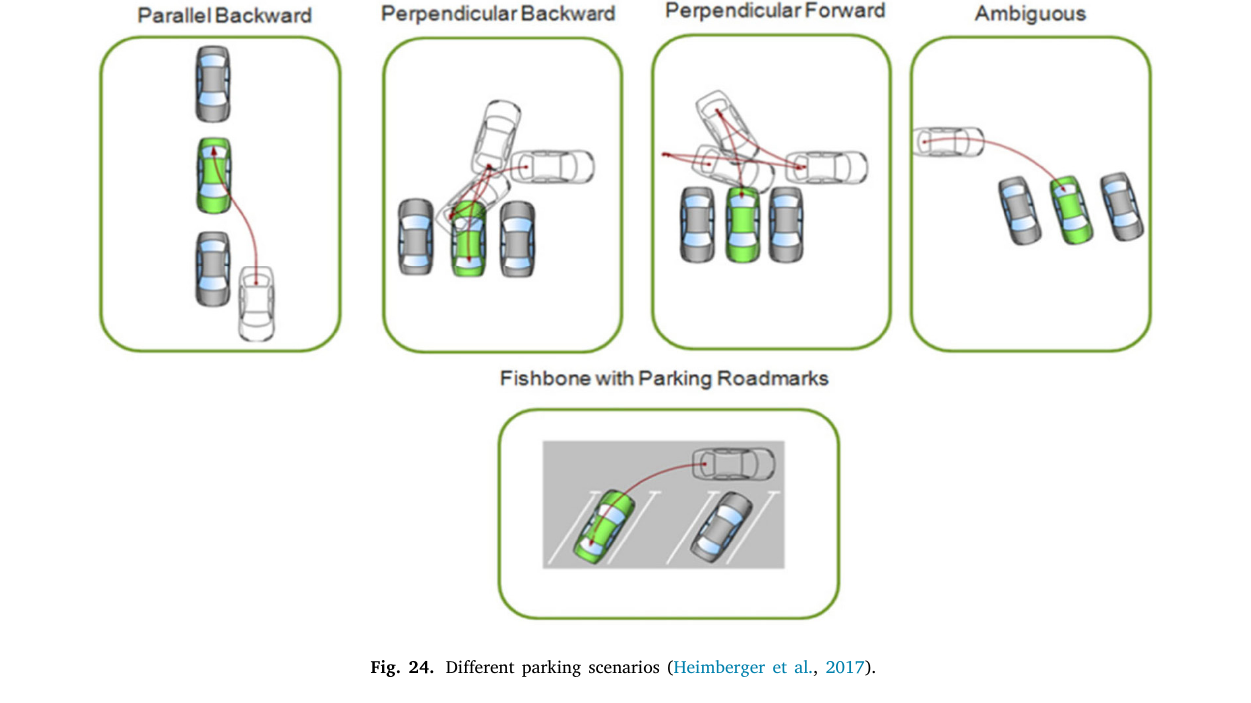
\includegraphics[width=0.6\textwidth]{img/15Screenshot_20231106_143633}\label{fig:15}
            \end{subfigure}
            \begin{subfigure}
                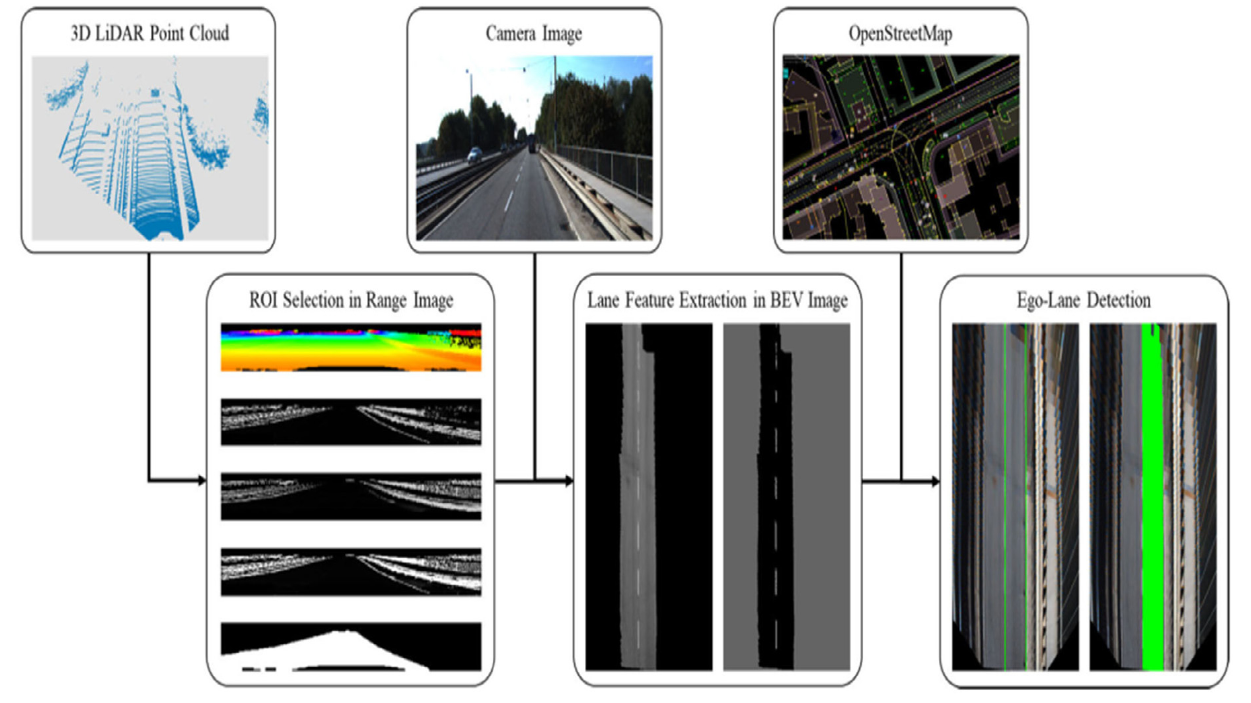
\includegraphics[width=0.9\textwidth]{img/14 Screenshot_20231106_143419}\label{fig:14}
            \end{subfigure}
            \begin{subfigure}
                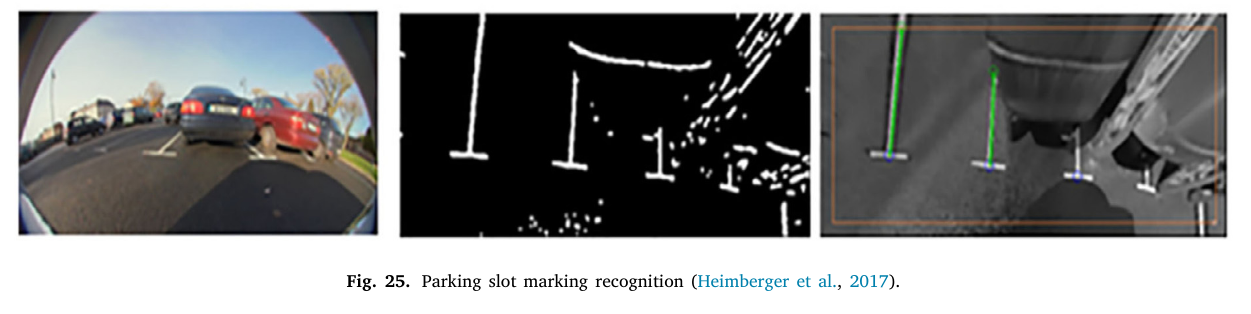
\includegraphics[width=0.8\textwidth]{img/16Screenshot_20231106_143701}\label{fig:16}
            \end{subfigure}
        \end{figure}
        \clearpage

        \hline
        \noindent \textbf{Referencia:}~\cite{althoff2009model} \\
        \textbf{Título:} \\
        Vision-based autonomous car racing using deep imitative reinforcement learning \\
        \textbf{Autores:}
        Cai, Peide and Wang, Hengli and Huang, Huaiyang and Liu, Yuxuan and Liu \\
        \textbf{Año:}
        2021 \\
        \textbf{Revista:}
        IEEE Robotics and Automation Letters \\
        \textbf{URL:}
        \url{https://ieeexplore.ieee.org/abstract/document/9488179} \\
        \textbf{Resumen:}
        \begin{itemize}
            \item El automovilismo autónomo es un desafío en el campo del control robótico, que históricamente ha requerido mapas precisos,
            localización y planificación, lo que lo hace computacionalmente ineficiente y sensible a cambios en el entorno.
            \item  Recientemente, se han desarrollado sistemas de aprendizaje profundo de extremo a extremo que muestran resultados prometedores
            en la conducción/racing autónoma.Sin embargo, estos sistemas suelen basarse en aprendizaje por imitación supervisada (IL),
            que enfrenta problemas de discrepancia en la distribución de datos.
            \item También se han utilizado métodos de aprendizaje por refuerzo (RL), pero requieren una gran cantidad de datos de interacción riesgosa.
            \item se presenta un enfoque general de aprendizaje profundo imitativo y de refuerzo (DIRL) que logra el automovilismo
            autónomo ágil utilizando entradas visuales.
            \item El conocimiento de conducción se adquiere tanto del aprendizaje por imitación como del aprendizaje basado en modelos de RL,
            permitiendo al agente aprender de instructores humanos y mejorar su rendimiento interactuando con un modelo de mundo offline.
            \item Se valida el algoritmo en una simulación de conducción de alta fidelidad y en un automóvil RC a escala 1/20
            en el mundo real con capacidad computacional limitada.
            \item  Los resultados de la evaluación muestran que el método supera a los enfoques anteriores de IL y RL en eficiencia
            de muestra y rendimiento en la tarea.
        \end{itemize} \\
        \hline
        \pagebreak
        \hline
        \noindent \textbf{Referencia:}~\cite{bachute2021autonomous} \\
        \textbf{Título:} \\
        Model-based probabilistic collision detection in autonomous driving \\
        \textbf{Autores:}
        Althoff, Matthias and Stursberg, Olaf and Buss \\
        \textbf{Año:}
        2009 \\
        \textbf{Revista:}
        IEEE Transactions on Intelligent Transportation Systems \\
        \textbf{URL:}
        \url{https://ieeexplore.ieee.org/abstract/document/4895669} \\
        \textbf{Resumen:} \\
        \begin{itemize}
            \item El artículo se centra en la seguridad de los caminos planificados para autos autónomos en relación con otros participantes en el tráfico.
            \item Se predice la ocupación de la carretera por otros vehículos de manera estocástica.
            \item La predicción tiene en cuenta las incertidumbres derivadas de las mediciones y los posibles comportamientos
            de los otros participantes en el tráfico.
            \item También se considera la interacción entre los participantes en el tráfico y las limitaciones de las maniobras
            de conducción debido a la geometría de la carretera.
            \item El resultado principal del enfoque presentado es la probabilidad de que ocurra un choque para una trayectoria específica de un auto autónomo.
            \item El enfoque se destaca por su eficiencia, ya que la mayoría de los cálculos intensivos se realizan de manera
            offline, lo que permite disponer de un algoritmo en línea eficiente para aplicaciones en tiempo real.
        \end{itemize} \\
        \hline
        \pagebreak
        \hline
        & \textbf{Referencia:}~\cite{cai2021vision}     \\
        \textbf{Título:} \\
        Motion Planning and Object Recognition Algorithms, Vehicle Navigation and Collision Avoidance Technologies,
        and Geospatial Data Visualization in Network Connectivity Systems \\
        \textbf{Autores:}
        Cai, Peide and Wang, Hengli and Huang, Huaiyang and Liu, Yuxuan and Liu \\
        \textbf{Año:}
        2022 \\
        \textbf{Revista:}
        IEEE Robotics and Automation Letters \\
        \textbf{URL:}
        \url{https://ieeexplore.ieee.org/abstract/document/9488179} \\
        & \textbf{Resumen en inglés:}                   \\
        & (Resumen en inglés para la referencia 4)      \\
        &                                               \\
        \hline
        & \textbf{Referencia:}~\cite{konecny2022motion} \\
        & \textbf{Resumen en inglés:}                   \\
        & (Resumen en inglés para la referencia 5)      \\
        &                                               \\
        \hline
        & \textbf{Referencia:}~\cite{li2022human}       \\
        & \textbf{Resumen en inglés:}                   \\
        & (Resumen en inglés para la referencia 6)      \\
        &                                               \\
        \hline
        & \textbf{Referencia:}~\cite{pavel2022vision}   \\
        & \textbf{Resumen en inglés:}                   \\
        & (Resumen en inglés para la referencia 7)      \\
        &                                               \\
        \hline
        & \textbf{Referencia:}~\cite{prasad2023design}  \\
        & \textbf{Resumen en inglés:}                   \\
        & (Resumen en inglés para la referencia 8)      \\
        &                                               \\
        \hline
        & \textbf{Referencia:}~\cite{sushma2023dynamic} \\
        & \textbf{Resumen en inglés:}                   \\
        & (Resumen en inglés para la referencia 9)      \\
        &                                               \\
        \hline
    \end{longtable}
%    \begin{itemize}
%        \item \cite{alam2022cost}
%        \item \cite{althoff2009model}
%        \item \cite{bachute2021autonomous}
%        \item \cite{cai2021vision}
%        \item \cite{konecny2022motion}
%        \item \cite{li2022human}
%        \item \cite{pavel2022vision}
%        \item \cite{prasad2023design}
%        \item \cite{sushma2023dynamic}
%    \end{itemize}
    \nocite{*}
    \bibliographystyle{acm}
    \bibliography{referecias}
\end{document}
